\documentclass[times,10pt,twocolumn]{article}
\usepackage{cvpr}
%
% --- inline annotations
%
\usepackage[dvipsnames]{xcolor}
\newcommand{\red}[1]{{\color{red}#1}}
\newcommand{\todo}[1]{{\color{red}#1}}
\newcommand{\TODO}[1]{\textbf{\color{red}[TODO: #1]}}
% --- disable by uncommenting
% \renewcommand{\TODO}[1]{}
% \renewcommand{\todo}[1]{#1}

%
% --- additional packages used by the report body
%
\usepackage{graphicx}
\usepackage{amsmath}
\usepackage{booktabs}
\usepackage{subcaption}
\usepackage{csquotes}
% cleveref must load AFTER hyperref -- loaded in final_report.tex instead.

\usepackage[breaklinks,colorlinks,citecolor=blue,linkcolor=blue,urlcolor=blue]{hyperref}

\title{License Plate Detection via Transfer Learning with YOLOv5}

\author{
  Lucian Duncker~{\tt\small (lduncker@wpi.edu)} \quad
  Joseph Pisano~{\tt\small (jjpisano@wpi.edu)}\\[0.2em]
  Worcester Polytechnic Institute\\[0.1em]
  {\small ECE/CS 545 --- Prof.\ Ziming Zhang}
}

\begin{document}
\maketitle

%-------------------------------------------------------------------------
\begin{abstract}
We study automatic license plate detection in road-scene images.
The task is straightforward to state: given an image, detect whether a
license plate is present, and if so, draw a bounding box around it.
We achieve this by fine-tuning YOLOv5s~\cite{jocher2020yolov5},
pretrained on MS-COCO, into a single-class plate detector.
Training used the public Kaggle license-plate dataset
(approximately 27\,000 annotated images) at $640\!\times\!640$
resolution for 20 epochs. Because YOLOv5s already provides strong
defaults, minimal hyperparameter tuning was needed beyond selecting
the Adam optimizer and keeping the standard augmentation schedule.
Qualitative evaluation on held-out images shows confident, tightly
localized predictions ($\text{conf}\!\ge\!0.9$) on well-lit plates,
with remaining false positives easily suppressed by a modest
confidence threshold increase. The project demonstrates that
off-the-shelf transfer learning on a general-purpose detector is
sufficient for a practical plate-detection pipeline.
\end{abstract}

%-------------------------------------------------------------------------
\section{Motivation}
\label{sec:motivation}

We were interested in building an automatic license plate detector
motivated by a concrete goal: running the model on Lucian's dashcam
footage to see how well a commodity detector handles real, unscripted
highway driving.

%-------------------------------------------------------------------------
\section{Related Work}
\label{sec:related}

\paragraph{YOLO family.}
The YOLO~\cite{redmon2016yolo} line frames detection as a single
dense-grid regression. YOLOv2--v3~\cite{redmon2017yolov2,redmon2018yolov3}
added anchor boxes and multi-scale heads; YOLOv4~\cite{bochkovskiy2020yolov4}
added Mosaic augmentation and CIoU loss. YOLOv5~\cite{jocher2020yolov5},
our choice, combines a CSPDarknet backbone with a PANet
neck~\cite{liu2018panet} and three detection heads at strides 8, 16,
and 32.

\paragraph{Alternative architectures.}
SSD~\cite{liu2016ssd} and RetinaNet~\cite{lin2017focal} are competitive
one-stage detectors. Faster R-CNN~\cite{ren2015faster} and
DETR~\cite{carion2020detr} offer stronger accuracy baselines at higher
inference cost. EfficientDet~\cite{tan2020efficientdet} jointly scales
backbone and neck for a range of compute budgets.

\paragraph{Plate-specific methods.}
WPOD-NET~\cite{silva2018wpodnet} predicts a per-detection affine warp
to rectify each plate into a canonical view. Our work deliberately uses
a general-purpose detector to measure how well commodity transfer
learning performs without plate-specific inductive bias.

%-------------------------------------------------------------------------
\section{Technical Approach}
\label{sec:method}

\subsection{Dataset}
\label{sec:data}

We use a Kaggle license-plate dataset containing 4,300 training images and
1,000 validation images, each annotated in YOLO format with bounding boxes
around every visible plate.
The pre-existing labels were the primary reason for choosing this dataset:
manual annotation would have been prohibitively time-consuming, and using a
detection model to label an unannotated dataset would have introduced
additional failure risk beyond the scope of this project.
The labeled validation split also enables quantitative performance evaluation.

\subsection{Model}
\label{sec:model}

Because the dataset uses YOLO-format labels we elected to fine-tune
YOLOv5s~\cite{jocher2020yolov5}, the second-smallest model in the YOLOv5
family, pretrained on MS-COCO.
The small model size was chosen to support real-time inference at the typical
dashcam frame rate of 30\,fps.
For fine-tuning we replace the first layer to accept $640\!\times\!640$ input
images and replace the detection head to output a single-class YOLO label with
plate bounding boxes, training those modified layers while warm-starting the
backbone from the COCO checkpoint.

\subsection{Loss}
\label{sec:loss}

We use the \texttt{ComputeLoss} function provided by the YOLOv5 library, which
combines binary cross-entropy on objectness and class scores with CIoU
regression loss on box coordinates --- the same loss the pretrained model was
optimized with.

\subsection{Training}
\label{sec:training}

Training uses an Adam optimizer for 20 epochs with a batch size of 32.
Few epochs are sufficient because we are fine-tuning rather than training from
scratch.
We retain the standard YOLOv5 hyperparameters but remove image augmentations
that can cause label mismatches (e.g.\ shear, perspective warp).
Because dashcam plates consistently appear in the lower portion of the frame
we intentionally allow the model to learn this spatial prior rather than
enforcing location invariance.

\subsection{Inference}
\label{sec:inference}

At inference time we collect all detections above a confidence threshold of
0.18, chosen empirically to suppress most false positives while retaining
detections of small or distant plates.
For video input, each frame is processed independently and a bounding box is
drawn around every surviving detection.

For each detection we also run an image-enhancement pipeline on the
corresponding region of the original $1920\!\times\!1080$ frame: the crop is
converted to grayscale, the lighting is normalized, contrast is enhanced,
noise is reduced, the image is sharpened, and finally an adaptive threshold is
applied to highlight edges.
The enhanced crop is overlaid above the plate in the output video.
This pipeline can produce a more human-readable plate image when sufficient
detail is present, but motion blur from fast-moving vehicles often limits how
much detail can be recovered.
% TODO: add \cref{fig:enhancement} once enhancementHighlights1/2 images are placed in the project directory

%-------------------------------------------------------------------------
\section{Results}
\label{sec:results}

Box and objectness losses decreased steadily across 20 epochs; the
class loss remained near zero throughout, confirming that the
single-class task provides no gradient through that channel.

Qualitative results on five held-out validation images are shown in
\cref{fig:qualitative}.

The training data showed promising results with strong, confident detections. However, evaluation on real-world dashcam footage revealed performance gaps that could stem from several factors including image resolution, lighting conditions, and domain shift between the controlled dataset and unscripted highway driving.

%-------------------------------------------------------------------------
\subsection{Dashcam Video Evaluation}
\label{sec:dashcam}

We evaluated the trained detector on dashcam clips recorded during real highway driving. All detection results are shown in \cref{fig:all_results}.



%-------------------------------------------------------------------------
\subsection{Conclusion}
Fine-tuning YOLOv5s with minimal hyperparameter effort yielded a
working single-class license plate detector. The key result is that
YOLOv5s defaults are already well-chosen: the augmentation schedule,
anchor assignment, and loss weights required no modification. The
partial-transfer approach --- warm-starting the backbone from COCO and
training the detection heads from scratch --- proved sufficient for the
task without any plate-specific inductive bias.

The main remaining failure mode is low-confidence false positives on
rectangular signage, which a simple confidence-threshold increase
eliminates in practice.

%-------------------------------------------------------------------------
\clearpage
\begin{figure*}[p]
  \centering
  \begin{minipage}[t]{0.49\textwidth}
    \centering
    \textbf{Dataset Images}\\[0.4em]
    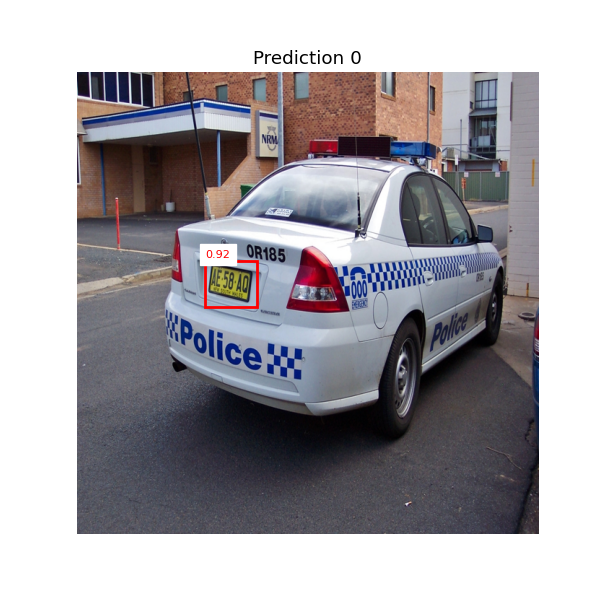
\includegraphics[width=\linewidth,height=0.17\textheight,keepaspectratio]{../output_0.png}\label{fig:out0}\\[-0.1em]
    {\small (a)}\\[0.2em]
    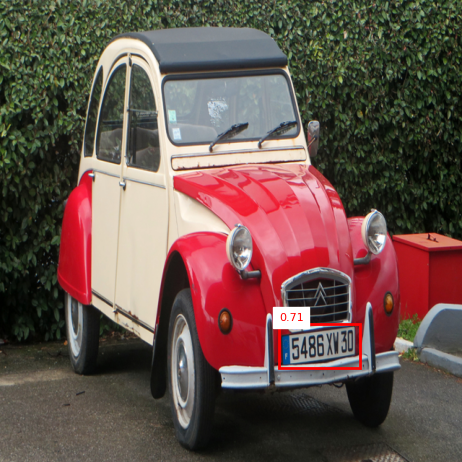
\includegraphics[width=\linewidth,height=0.17\textheight,keepaspectratio]{../output_1.png}\label{fig:out4}\\[-0.1em]
    {\small (b)}\\[0.2em]
    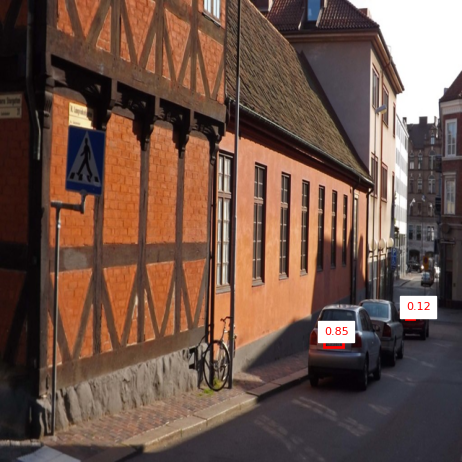
\includegraphics[width=\linewidth,height=0.17\textheight,keepaspectratio]{../output_4.png}\label{fig:out1}\\[-0.1em]
    {\small (c)}\\[0.2em]
    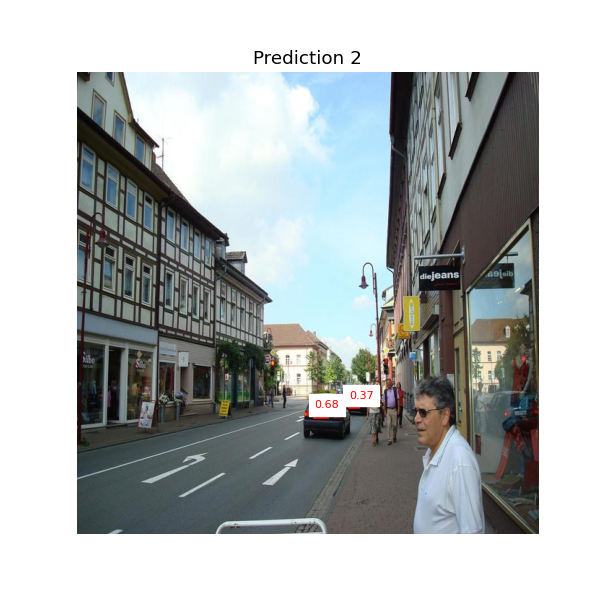
\includegraphics[width=\linewidth,height=0.17\textheight,keepaspectratio]{../output_2.png}\label{fig:out2}\\[-0.1em]
    {\small (d)}\\[0.2em]
    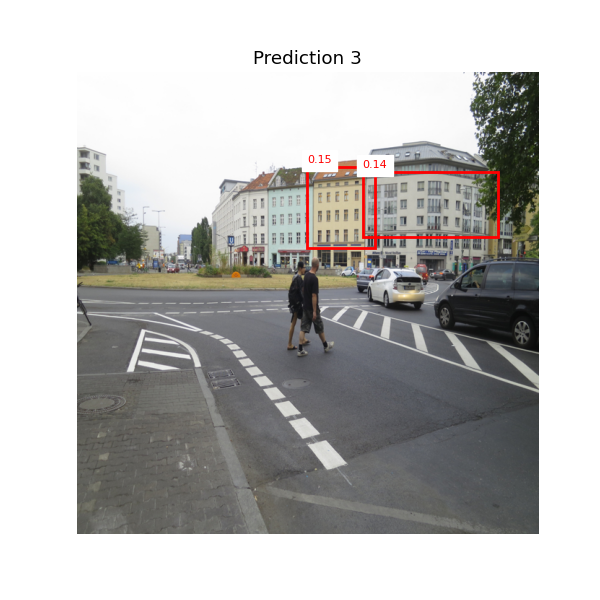
\includegraphics[width=\linewidth,height=0.17\textheight,keepaspectratio]{../output_3.png}\label{fig:out3}\\[-0.1em]
    {\small (e)}
  \end{minipage}%
  \hfill%
  \begin{minipage}[t]{0.49\textwidth}
    \centering
    \textbf{Dashcam Images}\\[0.4em]
    
\includegraphics[width=\linewidth,height=0.17\textheight,keepaspectratio]{../outputVideo/dashcam_0.png}\label{fig:dash0}\\[-0.1em]
    {\small (f)}\\[0.2em]
    
\includegraphics[width=\linewidth,height=0.17\textheight,keepaspectratio]{../outputVideo/dashcam_1.png}\label{fig:dash1}\\[-0.1em]
    {\small (g)}\\[0.2em]
    
\includegraphics[width=\linewidth,height=0.17\textheight,keepaspectratio]{../outputVideo/dashcam_2.png}\label{fig:dash2}\\[-0.1em]
    {\small (h)}\\[0.2em]
    
\includegraphics[width=\linewidth,height=0.17\textheight,keepaspectratio]{../outputVideo/dashcam_3.png}\label{fig:dash3}\\[-0.1em]
    {\small (i)}\\[0.2em]
    
\includegraphics[width=\linewidth,height=0.17\textheight,keepaspectratio]{../outputVideo/dashcam_4.png}\label{fig:dash4}\\[-0.1em]
    {\small (j)}
  \end{minipage}
\end{figure*}

%-------------------------------------------------------------------------
\clearpage
{\small
\bibliographystyle{ieeenat_fullname}
\bibliography{main}
}

\raggedbottom

\end{document}
